\documentclass[tikz,border=6pt]{standalone}
\usetikzlibrary{arrows.meta}
\definecolor{red}{HTML}{A50F2D}\definecolor{ink}{HTML}{141414}\definecolor{gry}{HTML}{5F5F5F}
\begin{document}
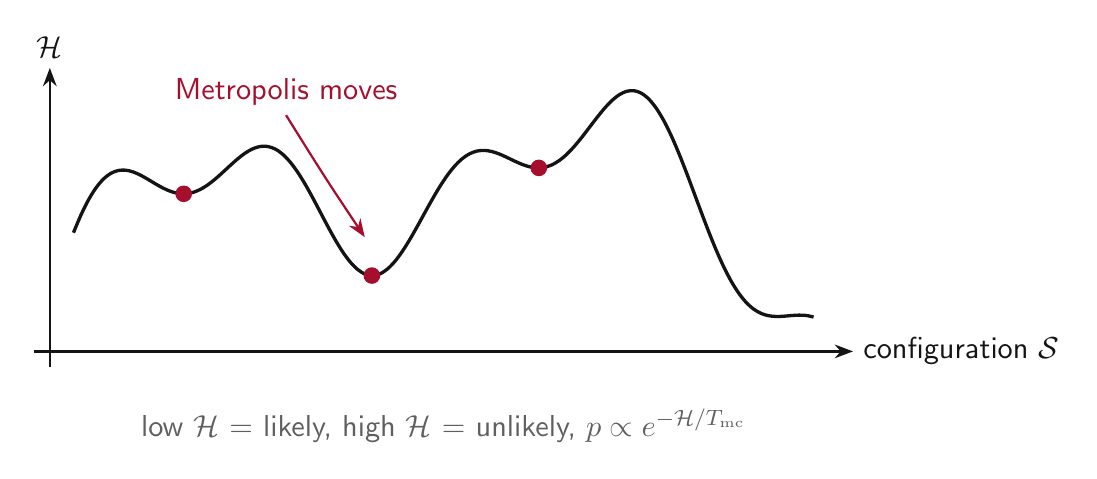
\begin{tikzpicture}[font=\sffamily\fontsize{11}{13}\selectfont,>=Stealth]
\draw[->,ink,thick] (-0.2,0)--(10.2,0) node[right]{configuration $\mathcal{S}$};
\draw[->,ink,thick] (0,-0.2)--(0,3.6) node[above]{$\mathcal{H}$};
\draw[ink,very thick,smooth,samples=100,domain=0.3:9.7] plot (\x,{1.5+0.9*sin(deg(\x*1.1))+0.5*sin(deg(\x*2.7))-0.07*(\x-5)*(\x-5)+0.9});
% states
\foreach \x in {1.7,4.09,6.21}{\fill[red] (\x,{1.5+0.9*sin(deg(\x*1.1))+0.5*sin(deg(\x*2.7))-0.07*(\x-5)*(\x-5)+0.9}) circle (3pt);}
\draw[red,->,thick] (3.0,3.0) .. controls (3.5,2.2) .. (4.0,1.45);
\node[red,anchor=south] at (3.0,3.0) {Metropolis moves};
\node[gry,anchor=north] at (5,-0.6) {low $\mathcal{H}$ = likely, high $\mathcal{H}$ = unlikely, $p\propto e^{-\mathcal{H}/T_{\mathrm{mc}}}$};
\end{tikzpicture}
\end{document}
